% !TeX spellcheck = en_US
\addsection{Player Turns}{\spells/dimension_door.png}

\begin{multicols*}{2}

At the start of a player's Turn, that player refreshes their hand of Cards from their Deck of Might \& Magic following two steps in order:
\begin{itemize}
  \item Discard any number of Cards from your hand.
If your current hand exceeds your Hand Limit \includesvg[height=10px]{\svgs/hand.svg}, you must discard down to at least your Hand Limit.
  \item Draw back to your Hand Limit.
\end{itemize}
Your current Hand Limit depends on your Main Hero's \hyperlink{Level}{Level}.
The beginning of your Turn is the only time your Hand Limit is checked.\par
There are three types of Actions players may take during their turn: \textbf{Movement}, \textbf{Town} and \textbf{Morale} Actions.
Once all players have spent all their Movement Points on their Turns and do not wish to use any further Town or Morale Actions, the current Round is over.
\subsection*{Movement Actions}
\hypertarget{Movement}{Movement Actions} are performed by spending Movement Points.
A player can use Movement Actions \textbf{only during their own Turn}.\par
For every 1 MP spent, you can perform one of the following Actions:
\begin{itemize}
  \item Move a Hero 1 Field in any direction.
  \item \hyperlink{Categories}{Re-visit} a Field where your Hero is in.
  \item \hyperlink{Timelimit}{Continue Combat} against Neutral Units for 1 additional Combat Round.
  \item \hyperlink{Placing}{Discover a face down Map Tile} if your Hero is on a Field next to that Tile.
  \item Place a new Map Tile from your pool of Far (II-III) Map Tiles.
\end{itemize}

\begin{center}
  \includesvg[width=0.6\linewidth]{\images/movement_tokens.svg}\\
  \medskip
  \footnotesize\textit{An active and an inactive Movement Token.}
\end{center}

\bigskip

Mark the amount of MP you have used by flipping your Movement Tokens over to their brown, inactive side.
If a player has both a Main and a \hyperlink{Secondary}{Secondary Hero}, track their MP separately.
Heroes can spend MP in any order.\par
Allied Heroes can move through each other but cannot stop their movement in the same Field.
When you move through a Field with an allied Hero, do not \hyperlink{Categories}{visit} the Field that the allied Hero is standing on.
In the unlikely situation that two allied Heroes are forced onto the same Field, you must use your next MP to move one of them away from that Field.\par
\textbf{Important}: Whenever you are instructed to gain (additional) MP, sometimes shorthanded with the symbol \includesvg[height=10px]{\svgs/movement.svg}, that MP persists for \textbf{only the Turn it was gained on}.
In the unlikely situation that two allied Heroes are forced onto the same Field, you must use your next MP to move one of them away from that Field.

\subsection*{Town Actions}
You can perform each of the Town Actions listed below \textbf{once per Round}.
These Actions can be performed at any point during any player's turn, except during Combat or when a player is resolving an Action that would be interrupted by your Town Action.
For example, you cannot draw Spell cards simultaneously with the Spell Book Token.\par
When a player announces that they are about to start Combat, you may react to it with any number of Town Actions before performing any of the steps of \hyperlink{Combatsetup}{setting up Combat.}\par
If multiple players wish to use a Town Action at the same time and the order of resolving them has an effect on the game, you may roll an Attack or Resource Die and let the highest roller perform the Action first.\par
After performing a Town Action, flip the respective Token on its inactive side on your Town Board.
You cannot use that action again until the start of the next Round, when the Tokens are refreshed.
\begin{itemize}
  \item [{
\includegraphics[height=1.5\baselineskip, valign=c]{\images/build.png}}] Build Token, used to expand your \hyperlink{Town}{Town}.
  \item [{
\includegraphics[height=1.5\baselineskip, valign=c]{\images/population.png}}] Population Token, used to Recruit and Reinforce \hyperlink{Units}{Units} or to Recruit \hyperlink{Secondary}{a Secondary Hero}.
  \item [{
\includegraphics[height=1.5\baselineskip, valign=c]{\images/spells.png}}]Spell Book Token, used to purchase \hyperlink{spells}{Spells}.
\end{itemize}

\subsection*{Morale Actions}
Players can gain or lose Morale through various game effects.
When you gain Morale, place a Positive Morale Token \includesvg[height=10px]{\svgs/positive.svg} near your play area.
A player may only have one such token.
If they would gain a second token, they may immediately spend the first one before gaining the second.
A Positive Morale Token may be spent to perform any of the following Actions at any time:
\begin{itemize}
  \item Draw a Card from your Deck.
  \item Discard any number of Cards, then draw that many Cards.
  \item Reroll any die you have thrown.
\end{itemize}

If a player loses Morale, they must discard a Positive Morale Token \includesvg[height=10px]{\svgs/positive.svg} without effect if they have one, otherwise they gain a Negative Morale Token \includesvg[height=10px]{\svgs/negative.svg}.
Inversely, gaining Morale while you have a Negative Morale Token also discards it without effect.
If a player would gain a second Negative Morale Token, they must instead discard their entire hand of Cards the next time they end their Turn.\par
\textbf{NOTE:} The Necropolis \includesvg[height=10px]{\svgs/necro.svg} Faction ignores any Morale effects.
They cannot ever gain or lose Morale for any reason.

\vspace*{\fill}

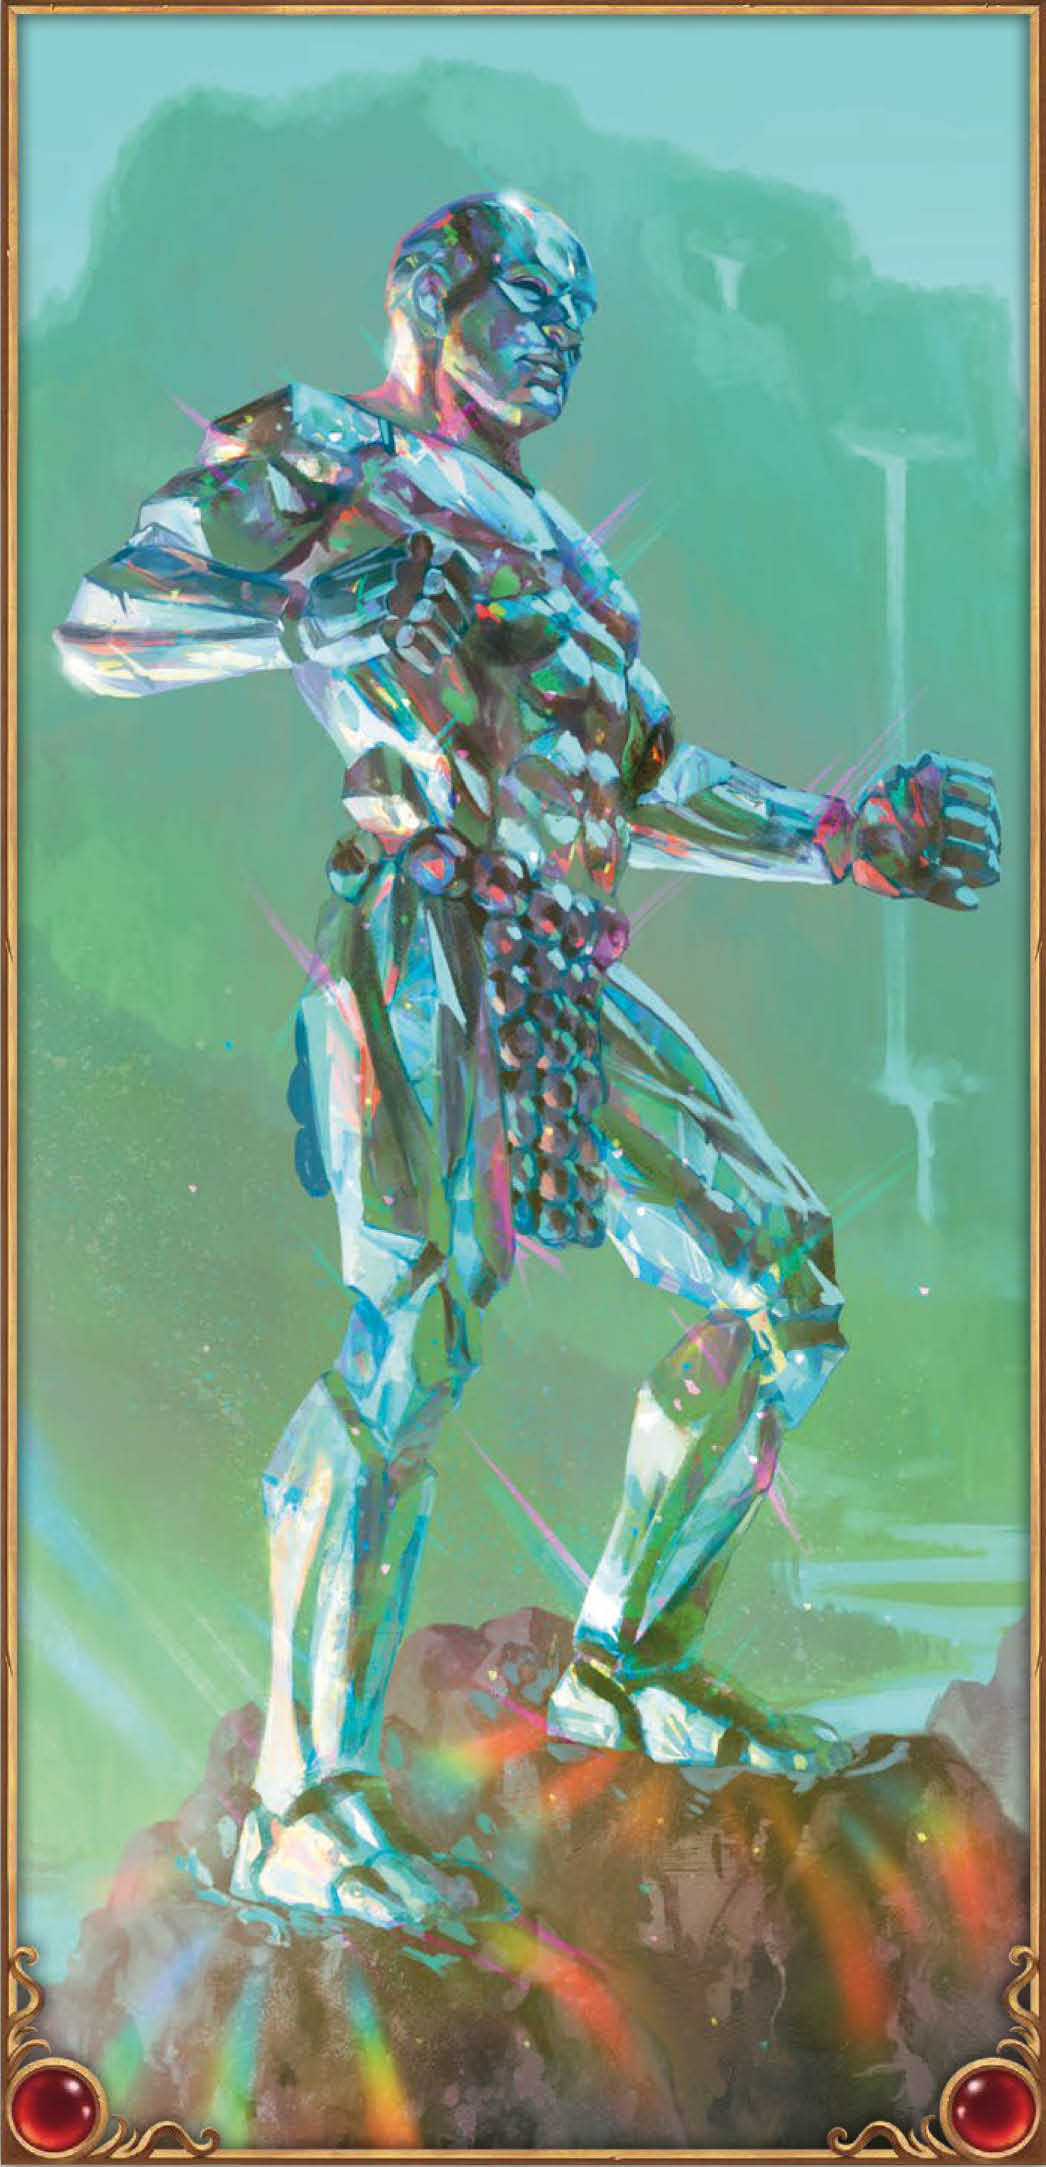
\includegraphics[width=\linewidth]{\art/diamond_golem.jpg}

\vspace*{\fill}

\end{multicols*}
